\documentclass{ks-pset}

\usepackage{ks-cs}

\newcommand\NP{\ensuremath{\mathbf{NP}}}
\newcommand\VC{\ensuremath{\text{\normalfont\textsc{Vertex Cover}}}}
\newcommand\Partition{\ensuremath{\text{\normalfont\textsc{Partition}}}}

\title{Homework 8}
\date{2022 April 20 (Wednesday)}
\author{}

\begin{document}

\begin{problem}[Shodoku!, 35]

  Many puzzles can be solved by transforming (or ``reducing'') them to network
  flow problems.  That's what you'll do here!

  ShoGames, a provider of popular online games, has developed a board game that
  works like this:  We're given an \(n×n\) board.  Some of the squares are gray
  and the rest are white.  The goal is to place \(n\) tokens on white cells such
  that every row contains exactly one token and every column contains exactly
  one token.  Tokens may not be placed on the gray cells.  For example,
  \cref{fig:board-game} shows a board with a valid placement of tokens
  (indicated by the X marks).

  \begin{center}
    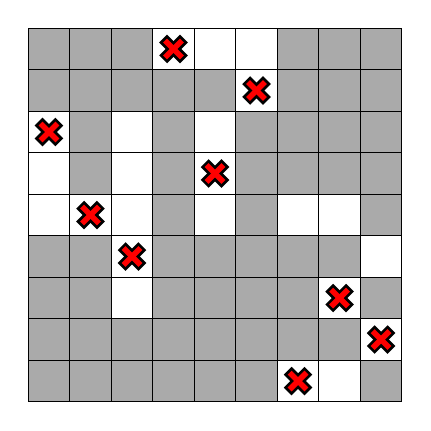
\begin{tikzpicture}[x=1.5em, y=1.5em]

      \tikzset{
        token outline/.style={
          line width=4pt,
          draw=black,
        },
        token/.style={
          line width=2pt,
          shorten <=1pt,
          shorten >=1pt,
          draw=red,
        },
        token/.pic={
          \foreach \style in {token outline,token} {
            \draw[\style] (1/4,1/4) -- (3/4,3/4);
            \draw[\style] (1/4,3/4) -- (3/4,1/4);
          }
        },
      }

      \fill[opacity=1/3, even odd rule]
      (0,0) -| (6,1) -| (8,0) -| (9,1) -| (8,2) -| (9,3) -| (8,4) -| (9,9) -|
      (6,7) -| (5,8) -| (3,9) -| (0,7) -| (1,5) -| (2,7) -| (3,2) -| (2,4) -| cycle
      (4,4) rectangle (5,7) (7,2) rectangle (8,3) (6,4) rectangle (8,5);

      \draw (0,0) grid[step=1] (9,9);

      \foreach \x/\y in {0/6,1/4,2/3,3/8,4/5,5/7,6/0,7/2,8/1} {
        \pic at (\x,\y) {token};
      }

    \end{tikzpicture}
    \captionof{figure}{A square board with a valid placement of tokens.}
    \label{fig:board-game}
  \end{center}

  You may assume that the board is represented as follows:  We're given the
  value of \(n\) (the width and height to the board) and a list of ordered
  pairs, each representing the row and column of a white cell in the board.
  Using existing graph algorithms, describe an efficient algorithm that
  determines whether or not a given board has a valid solution.  (You don't need
  to actually give the valid solution if it exists, although you'll see that
  this is not hard once you can determine whether or not a solution exists.)
  Prove that your algorithm is correct and derive its running time as a function
  of \(n\) (and only \(n\)---do not include other terms in the running time).

\end{problem}

\begin{solution}

  \paragraph{Self-assessment}

\end{solution}

\begin{problem}[The Big Difference Between Two and Three!, 35]

  In class we showed that the \VC{} decision problem is \NP-hard.
  \begin{subproblems}

    \item Show that the \VC{} decision problem can be solved in polynomial time
      if every vertex has degree at most \(2\).  Describe an algorithm, briefly
      explain why it is correct, and analyze its running time.  (You may be
      generous in your analysis, but make sure it's polynomial time.  Note also
      that the graph is not necessarily connected; it may comprise one or more
      connected components.)  \emph{A few sentences should suffice here.}

    \item Show that the \VC{} decision problem remains \NP-hard even if every
      vertex has degree at most \(3\).  It can be very helpful to use a diagram
      to help explain the construction.

  \end{subproblems}

\end{problem}

\begin{solution}

  \paragraph{Self-assessment}

\end{solution}

\begin{problem}[More \NP-Hardness!, 30]

  Let \(S=\Set{a₁,\dotsc,aₙ}\) and let \(f\colon S→ℤ₊\) (that is, \(f\) maps
  elements of \(S\) to the positive integers).  A \emph{partition} of \(S\) is a
  pair of sets \(A,B\) such that \(S=A∪B\) and \(A∩B=∅\).  The \Partition{}
  Problem asks if there exists a partition of \(S\) into sets \(A,B\) such that
  \[
    ∑_{x∈A}f(x)=∑_{x∈B}f(x).
  \]
  Notice that while this definition of the problem looks weird, it's written in
  this way in order to permit us to have multiple items with the same value,
  that is  a ``multiset'' of numbers.  Prove that \Partition{} is \NP-hard.

\end{problem}

\begin{solution}

  \paragraph{Self-assessment}

\end{solution}

\end{document}
